% File: PolygonNormal.tex
% Author: Adam Leeper
%------------------------------------------------------------------------------
\providecommand{\isolatedBuild}[1]{#1}% Fallback definition to build normally.
\isolatedBuild{
  \documentclass[11pt,letterpaper]{book}
  %\documentclass[11pt,letterpaper]{book}

% aleeper: I think these are needed for Paul's macros?
\usepackage{epsfig}
\usepackage{epstopdf}

%\makeatletter
%\typeout{The import path is \import@path}
%\makeatother

\usepackage{import}

\subimport{./}{packagesMitiguy.sty}
\subimport{./}{macrosMitiguy.tex}
\subimport{./}{PageStylesMitiguy.tex}
\subimport{./}{macrosLeeper.tex}
   % Found via TEXINPUTS environment variable.
  \isolatedBuildHeader{Vector Equations and Geometry}
                      {Polygon Meshes in Engineering and Graphics}
}
%%%
%%%
%%%
\begin{minipage}[t]{0.68\columnwidth}
  \minipageTopAnchor
  In many engineering applications -- such as stress and aerodynamics
  computations using finite elements, as well as CAD and graphical display --
  objects are represented using a group of polygons (usually triangles)
  collectively called a ``mesh". Being able to compute a ``normal'' vector
  perpendicular to each polygon is important for all these applications.
\end{minipage}
%
\hfill
%
\begin{minipage}[t]{0.25\columnwidth}
  \minipageTopAnchor
  \flushright
  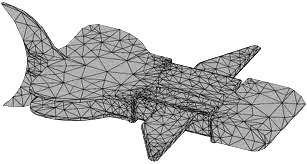
\includegraphics[width=0.9\columnwidth]{wing_robot.jpg}
\end{minipage}
%
\\[0.45pc]
In the figure below, the position vector to each vertex from \origin{A} is
labeled as a tuple of \uvecxyz{a} measures.
\\[0.0pc]
For example, $P_1 \equals[\;] (3, 2, 0)$ means
$\posvec{\origin{A}}{P_1} \equals[\;] 3~\uvecx{a} \plus[\;] 2~\uvecy{a}
\plus[\;] 0~\uvecz{a}$.
%
\begin{center}
  \includegraphicsAB[width=7cm]{polygon-solution.png}{polygon_normal.png}
\end{center}
%
\begin{enumerate}
  \item \underline{Compute} a vector \bvec{n} that is perpendicular to the
    polygon, expressed in terms of \uvecxyz{a}.
    \\[0.25pc]\textbf{Result:} \\[-1.0pc]
    %
    \begin{displaymath}
      \bvec{n} \equals[\;]
      \hidemath[2cm]{4~\uvecx{a} \plus[\;] 6~\uvecy{a} \plus[\;] 8~\uvecz{a}}
    \end{displaymath}
    %
    \Solution{}{0.98\linewidth}{
      \begin{tabular}{p{0.03\linewidth}ll}
        $\bvec{n}$
        & $\equals[\;] \posvec{P_1}{P_2} \CrossProduct[\;] \posvec{P_1}{P_3}$
        \\[0.45pc]
        %\begin{align*}
        $\posvec{P_1}{P_2}$
        & $\equals[\;] \posvec{\origin{A}}{P_2} \minus[\;] \posvec{\origin{A}}{P_1}$
        & $\equals[\;] (2 - 3)~\uvecx{a} \plus[\;] (0 - 2)~\uvecy{a}
        \plus[\;] (2 - 0)~\uvecz{a}$
        \\[0.45pc]
        & & $\equals[\;] -1~\uvecx{a} \minus 2~\uvecy{a} \plus[\;] 2~\uvecz{a}$
        %\end{align*}
        \\[0.45pc]
        $\posvec{P_1}{P_3}$
        & $\equals[\;] \posvec{\origin{A}}{P_3} \minus[\;] \posvec{\origin{A}}{P_1}$
        & $\equals[\;] (6 - 3)~\uvecx{a} \plus[\;] (0 - 2)~\uvecy{a}
        \plus[\;] (0 - 0)~\uvecz{a}$
        \\[0.45pc]
        & & $\equals[\;] 3~\uvecx{a} \minus 2~\uvecy{a}$
        \\[0.45pc]
        $\bvec{n}$
        & $\equals[\;] \posvec{P_1}{P_2} \CrossProduct[\;] \posvec{P_1}{P_3}$
        & $\equals[\;] (-1~\uvecx{a} \minus 2~\uvecy{a} \plus[\;] 2~\uvecz{a})
        \CrossProduct[\;] (3~\uvecx{a} \minus 2~\uvecy{a})$
        \\[0.45pc]
        & & $\equals[\;] -3~\uvecx{a} \CrossProduct[\;] ~\uvecx{a} \plus[\;]
        2~\uvecy{a} \CrossProduct[\;] ~\uvecx{a} \minus[\;] 6~\uvecy{a}
        \CrossProduct[\;] ~\uvecx{a} $
        \\[0.45pc]
        & & \quad\; $\plus[\;] 4~\uvecy{a} \CrossProduct[\;] ~\uvecy{a} \plus[\;]
        6~\uvecz{a} \CrossProduct[\;] ~\uvecx{a} \minus[\;] 4~\uvecz{a} \CrossProduct[\;] ~\uvecy{a}$
        \\[0.45pc]
        & & $\equals[\;] 2~\uvecz{a} \minus 6(-~\uvecz{a}) \plus[\;] 6~\uvecy{a}
        \minus 4(-~\uvecx{a})$
        \\[0.45pc]
        & & $\equals[\;] 4~\uvecx{a} \plus[\;] 6~\uvecy{a} \plus[\;] 8~\uvecz{a}$
      \end{tabular}
      \\[4.0pc]
    }
  \item \underline{Explain} in detail how to get \uvecHat{n}, the unit vector
    in the same direction as \bvec{n}. \boldDarkBlue{\underline{Sketch}}
    \uvecHat{n} on the figure.
    \\[0.45pc]
    %
    \Solution{}{0.98\linewidth}{
      To get \uvecHat{n}, simply divide \bvec{n} by its magnitude:
      $$\uvecHat{n} \equals[\;] \frac{\bvec{n}}{\magnitude{\bvec{n}}} \equals[\;]
      \frac{\bvec{n}}{\sqrt{\bvec{n}\CrossProduct[\;]\bvec{n}}}$$
      \\[-0.5pc]
    }
  %
  \item What is the geometric interpretation of the length of \bvec{n}?
    \\[0.45pc]
    %
    \Solution{}{0.98\linewidth}{
      The length of $\bvec{n}$, given by $\magnitude{\bvec{n}}$, is twice the
      area of the triangle shown.
      \\[0.25pc]
    }
\end{enumerate}
%
\isolatedBuildFooter
